

\documentclass[border=10pt,12pt]{standalone}
\usepackage[siunitx]{circuitikz} % Loading circuitikz with siunitx option
\begin{document}

\def\flipflop#1#2{
	\begin{scope}[shift={#1}, rotate=#2]
		\draw [fill=white,ultra thick](0,0) rectangle (1.5,2);
		\draw (0,0.5)--(0.2,0.6)--(0,0.7);
		\node at (0.2,1.5){D};
		\node at (1.2,1.5){Q};
	\end{scope}
}
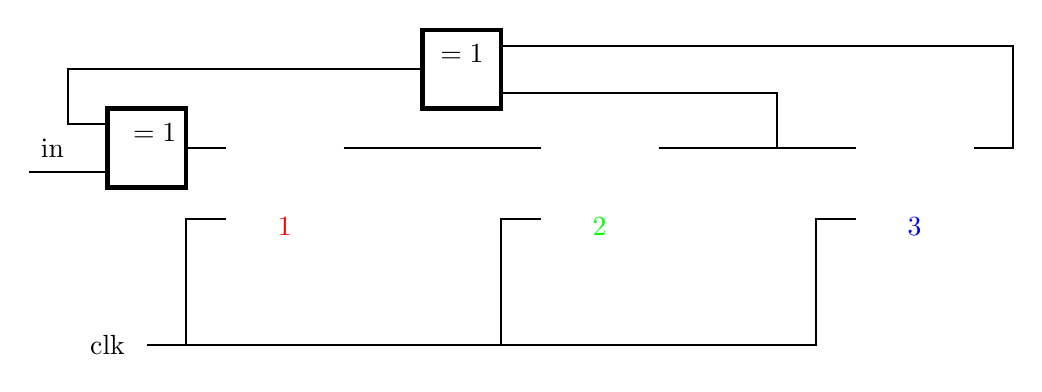
\begin{tikzpicture}
%Drawing the flipflops
	\flipflop{(0,0)}{0};
	\flipflop{(4,0)}{0};
	\flipflop{(8,0)}{0};
%drawing the xor gatter
	\draw [fill=white,ultra thick](-1.5,1) rectangle (-0.5,2);
	\node at (-0.9,1.7){$=1$};
	
	\draw [fill=white,ultra thick](2.5,3) rectangle (3.5,2);
	\node at (3,2.7){$=1$};

%connections
	\draw[thick] (0,0.6)--(-0.5,0.6)--(-0.5,-1)--(7.5,-1)--(7.5,0.6)--(8,0.6);
	\draw[thick] (-1,-1)--(-0.5,-1);
	\draw[thick] (-1,-1)--(-0.5,-1);
	\draw[thick] (4,0.6)--(3.5,0.6)--(3.5,-1);
	\draw[thick] (-0.5,1.5)--(0,1.5);
	\draw[thick] (1.5,1.5)--(4,1.5);
	\draw[thick] (5.5,1.5)--(8,1.5);
	\draw[thick] (9.5,1.5)--(10,1.5)--(10,2.8)--(3.5,2.8);
	\draw[thick] (7,1.5)--(7,2.2)--(3.5,2.2);
	\draw[thick] (-1.5,1.2)--(-2.5,1.2);
	\draw[thick] (-1.5,1.8)--(-2,1.8)--(-2,2.5)--(2.5,2.5);
	
	
% nodes for inputs
	\node at (-1.5,-1){clk};
	\node at (-2.2,1.5){in};
	\node[thick, color=red] at (0.75,0.5) {1};
	\node[thick, color=green] at (4+0.75,0.5) {2};
	\node[thick, color=blue] at (8+0.75,0.5) {3};
	
\end{tikzpicture}
\end{document}